\section{Results on Persuasiveness}
\label{sec:pers_results}

In this section, we analyze our results by showing a significant usage of linguistic features that resemble persuasive text (\S\ref{subsec:si_pers_corr}), showing generated text (\S\ref{subsec:si_pers_sample}), and with standard metrics (\S\ref{subsec:si_pers_auto}).  

\subsection{Linguistic Feature Correlations}
\label{subsec:si_pers_corr}

\Cref{fig:feature_correlations} shows the correlations between linguistic features and convincingness in the UKPConvArg1 corpus. The model details are in~\Cref{apx:lfc}.
% Persuasiveness Feature Correlations
\begin{figure}[h]
  \centering
  \caption{The correlations between linguistic features and convincingness in the UKPConvArg1 corpus. The lower x-axis is in the logit scale, and the percentage difference in odds of winning is on the upper x-axis. The figure is read as: if the feature for argument A is one standard deviation greater than the feature for argument B, the odds of A winning shift by the respective percent value. Notice that the correlations show a strong positive correlation with readability (\eg the Flesh score is positive while length and average syllables are negative). }
  \label{fig:feature_correlations}
  \scalebox{1.0}{
  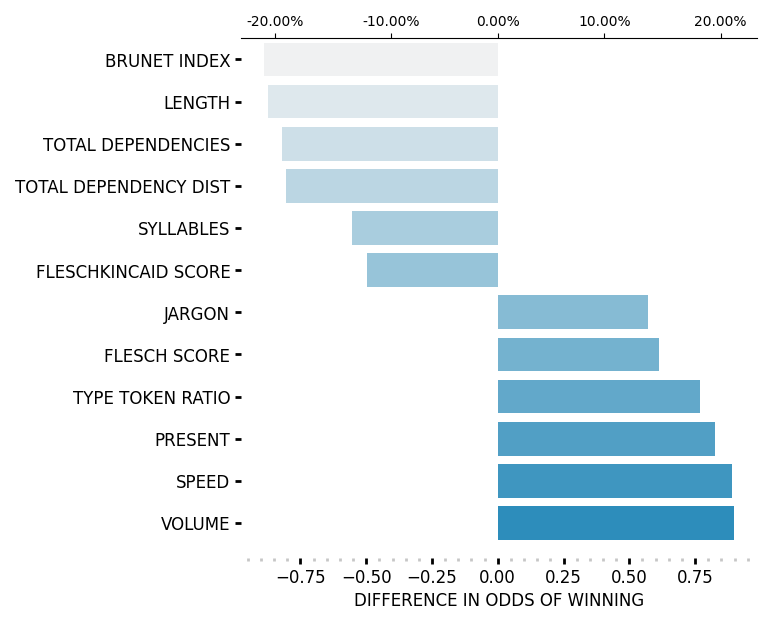
\includegraphics[width=\linewidth]{figs/16k_corr.png}
  }
\end{figure}

We find a strong positive correlation between readability and winning arguments. This is reflected by both readability scores (\eg SMOG, Flesch-Kincaid, etc.) and correlation with smaller words, fewer total dependencies, and a smaller overall total dependency distance. We notice a positive correlation with speed and volume. \citet{toubia-2021} define speed as the total distance covered by a text's word embeddings, normalized by the length of the text. Volume represents the amount of material covered by the text, calculated by estimating the volume enclosed by the word embeddings \citep{toubia-2021}. We also find a negative correlation with passive voice and a positive correlation with misspelled words (not shown for brevity).

We run a significance test to see how well our models learned the style (see~\Cref{apx:featureagreement}). Most models consistently learn pronounced trends (\ie Brunet index, length, speed, and volume). The augmented data likely led to this change because fine-tuning on the augmented set displays the same trends. In cases like total dependencies (TD) and the ratio of present tense verbs, models trained with the sample-dependent discriminator (SD) loss are significantly better at learning the trend, despite the data not actively showing the trend (or completely opposing it). In the case of Flesch score, models trained with SD loss can nullify the trend which occurs in the incorrect direction. This displays that models trained with the SD loss are substantially better at learning from the dataset than the baselines and models trained with the sample-dependent supervised (SS) loss. One example of failure is the ratio of jargon, likely because the model could not generate out of vocabulary words, but this is a limitation of how we define jargon.

% We also show the results of Table~\Cref{tab:feature-evaluation} in the context of the full feature set in the Appendix by computing an agreement score. 


\subsection{Sample Generations}
\label{subsec:si_pers_sample}



% Persuasiveness Sample Generations

  \begin{table}[htb]
  \small
  \centering
  \caption{The baseline models and our model (GPT2 with the SD loss and $\beta=0.5$ on the augmented data). The models are fed the input ``Plastic bottles are bad because'' and ``Gaming is good for child development because'', generating up to 100 tokens using beam search.}
  \label{tab:example_persuasive} 
  \begin{tabularx}{\linewidth}{@{}>{\raggedright\arraybackslash}X@{}}
   \toprule[1.5pt]
  \textsc{Model} \& \textsc{Generated Text}\\
  \midrule[0.75pt]
  \textsc{Example 1:}\\
  \textbf{GPT2}:  Plastic water bottles are bad because they are not recyclable," he said. "They are not good for the environment, they are not recyclable."  \\
  \textbf{GPT2-Aug}: Plastic water bottles are bad because it causes pollution. Also water bottles also cost more than regular water. \\
  \textbf{TStylist}: Plastic water bottles are bad because plastic water bottles are bad for our environment.\\
  \textbf{Ours (SD-0.5)}: Plastic water bottles are bad because they are not recycled and end up in landfills which lead to pollution of our environment. Plastic requires up to 47 million gallons of oil per year to produce.  \\
  \addlinespace[0.5em]
  \textsc{Example 2:}\\
  \textbf{GPT2}: Gaming is good for child development because it teaches them how to use a computer. It's good for the economy, it's good for the environment, it's good for the children, it's ...  \\
  \textbf{GPT2-Aug}: Gaming is good for child development because it allows the child to grow and develop. I believe eSports (LoL) should be a spectator sport and not a major part of the sports calendar.   \\
  \textbf{TStylist}: Gaming is good for child development because gaming is good for your child.\\
  \textbf{Ours (SD-0.5)}: Gaming is good for child development because it allows children to grow up in a world where they are exposed to a wide variety of ideas and experiences.   \\
  \bottomrule[1.5pt]\\
  \end{tabularx}
  \vspace{-10px}
  \end{table}


\Cref{tab:example_persuasive} shows the generations of three baselines and our best-performing method. We find that for both prompts, the generations of models trained with the sample-dependent discriminator (SD) loss generally have the highest values of speed, volume, and lexical diversity. For the second prompt, the speed and volume of our generation are larger than that of GPT2 and TStylist, but slightly smaller than that of GPT2 fine-tuned on the augmented data. Intuitively, this makes sense because the GPT-Aug generation covers much more information in the same time frame; however, this information isn't relevant to the argument, making our generation much more sensible. The baselines often suffer from neural degeneration, but the model trained with the SD loss does not face this issue. Since length had a strong negative correlation with persuasiveness, the model likely implicitly learned from the discriminator to handle this kind of neural degeneration. However, it is still an issue in some cases with out-of-domain samples.






% Persuasiveness ROUGE
  \begin{table}[htb]
  \centering
  \small
  \caption{ROUGE-\{1,2, L\} scores and BERT scores (F1) for all models. Baseline models: GPT2, GPT-2 fine-tuned on UKPConvArg1, GPT-2 with augmented data, TitleStylist \citep{jin2020hooks}. Our models are trained on augmented data and a sample-dependent discriminator (SD) or sample-dependent supervised (SS) loss with parameter $\beta$. The baseline ROUGE score increases due to data augmentation; the relevance of our models' generations is largely insensitive to loss type and parameter value.}
  \label{tab:automatic-evaluation}
  \scalebox{1.0}{
  \begin{tabularx}{0.9\linewidth}{@{}>{\raggedright\arraybackslash}Xcccc@{}}
   \toprule[1.5pt]
  \textsc{Model} & \textsc{RG-1}            & \textsc{RG-2}           & \textsc{RG-L}        &\textsc{B-F1} \\     
  \midrule[0.75pt]
  GPT2     & 0.1856          & 0.0968          & 0.1769         & 89.28          \\
  GPT2-UKP & 0.2474          & 0.1061          & 0.1989         & 87.21         \\
  GPT2-Aug & 0.2987          & 0.1845          & 0.2774         & 86.90          \\ 
  TStylist & 0.2578          & 0.1569          & 0.2391         & 84.70          \\ 
  \midrule[0.75pt]
  % \addlinespace[0.5em]
  SS-0.1   & 0.2925          & 0.1802          & 0.2717         & 88.95          \\
  SS-1.0   & 0.2862          & 0.1774          & 0.2634         & 89.18          \\
  SD-0.1  & 0.3036          & 0.1903          & 0.2802          & 88.75         \\
  SD-0.5  &    \textbf{0.3168} & \textbf{0.2296} & \textbf{0.3065 } & \textbf{89.56}       \\
  SD-0.8  & 0.2872          & 0.1957          & 0.2733          & 89.12         \\
  SD-1.0  & 0.2929          & 0.2224          & 0.2848          & 89.05         \\ 
  \bottomrule[1.5pt]\\
  \end{tabularx}
  }
  \vspace{-25pt}
  \end{table}
%   \begin{table}[htb]
  
%   \centering
%   \small
%   \caption{ROUGE-\{1,2, L\} scores for all models. Baseline models: GPT2, GPT-2 fine-tuned on UKPConvArg1, GPT-2 with augmented data, TitleStylist \citep{jin2020hooks}. Our models are trained on augmented data, and a sample-dependent discriminator (SD) or sample-dependent supervised (SS) loss with parameter $\beta$. The baseline ROUGE score increases due to data augmentation; the relevance of our models' generations is largely insensitive to loss type and parameter value.}
%   \label{tab:automatic-evaluation}
%   \scalebox{1.0}{
%   \begin{tabularx}{0.85\linewidth}{@{}>{\raggedright\arraybackslash}Xccc@{}}
%   \toprule[1.5pt]
%   \textsc{Model} & \textsc{RG-1}            & \textsc{RG-2}           & \textsc{RG-L} \\     
%   \midrule[0.75pt]
%   GPT2     & 0.1856          & 0.0968          & 0.1769                    \\
%   GPT2-UKP & 0.2474          & 0.1061          & 0.1989                   \\
%   GPT2-Aug & 0.2987          & 0.1845          & 0.2774                    \\ 
%   TStylist & 0.2578          & 0.1569          & 0.2391                    \\ 
%   \midrule[0.75pt]
%   % \addlinespace[0.5em]
%   SS-0.1   & 0.2925          & 0.1802          & 0.2717                    \\
%   SS-1.0   & 0.2862          & 0.1774          & 0.2634                    \\
%   SD-0.1  & 0.3036          & 0.1903          & 0.2802                    \\
%   SD-0.5  &    \textbf{0.3168} & \textbf{0.2296} & \textbf{0.3065 }         \\
%   SD-0.8  & 0.2872          & 0.1957          & 0.2733                    \\
%   SD-1.0  & 0.2929          & 0.2224          & 0.2848                    \\ 
%   \bottomrule[1.5pt]\\
%   \end{tabularx}
%   }
%   \vspace{-25pt}
%   \end{table}


\subsection{Automatic Metrics}
\label{subsec:si_pers_auto}
We compare the ROUGE scores of our experimental models in ~\Cref{tab:automatic-evaluation}, ensuring that the topics in the test set are not discussed anywhere in the UKPConvArg1 or augmented datasets. The data augmentation leads to a sharp increase in the ROUGE scores of the generations, showing that it is essential for robust and relevant generations. The results are relatively insensitive to variation in $\beta$ parameter that controls the tradeoff between reconstruction loss ($L_R)$ and discriminator loss ($L_R$). These scores show that our models generate relevant, but not necessarily persuasive, text. We find similar insights from the BERTScore; although the augmentation has a slight negative impact on the score, the difference is negligible. 

\section{Results on Memorability}
\label{sec:mem_results}

In this section, we focus on memorability and show that our model can generate more robust, relevant, and memorable text than the baselines. In~\Cref{subsec:si_mem_corr}, we find linguistic features that are strongly correlated with memorability. Then in~\Cref{subsec:si_mem_sample}, we show samples of generated text and lastly, in~\Cref{subsec:si_mem_auto}, we present the results on our automatic metrics.

\subsection{Linguistic Feature Correlations}
\label{subsec:si_mem_corr}
% Memorability Feature Correlations
% \begin{wrapfigure}{r}{0.5\textwidth}
\begin{figure}[t]

  \centering
  \caption{The correlations between linguistic features and persuasiveness in the Cornell Movie-Quotes Corpus. The lower x-axis is in the logit scale, and the percentage difference in odds of winning is on the upper x-axis. Notice that the correlations show a negative correlation with long and winding text (\ie circuitousness \citep{toubia-2021}). }
  \label{fig:mem_feature_correlations}
  \scalebox{1.0}{
    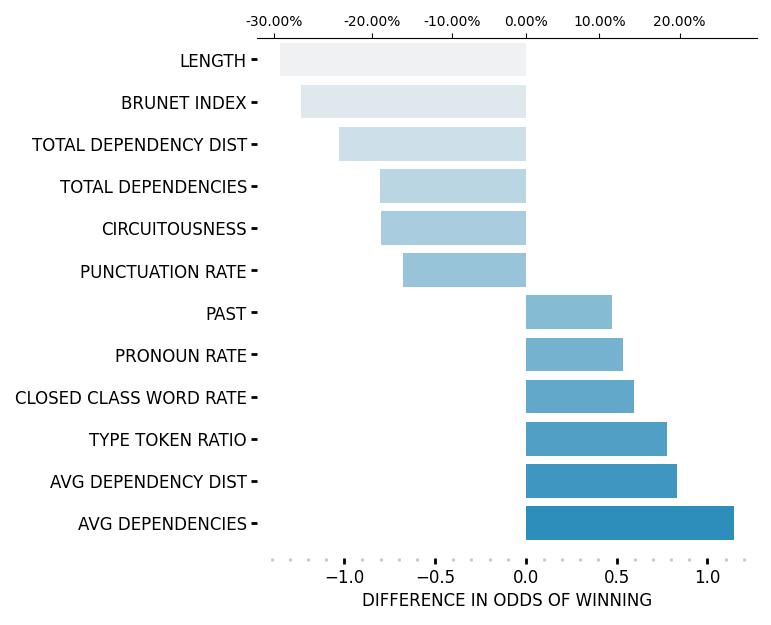
\includegraphics[width=\linewidth]{figs/imdb_corr.png}
  }
\end{figure}
% \end{wrapfigure}

We train a Bayesian hierarchical model for the Cornell Movie Quotes corpus, which produces the correlations shown in~\Cref{fig:mem_feature_correlations}. We find a strong negative correlation with long, winding text, shown by the trends in total dependencies, total dependency distance, length, and circuitousness. A higher circuitousness implies that a less direct route was taken to convey information \citep{toubia-2021}. Circuitousness is detrimental to memorability as winding text tends to be harder to remember. The negative correlation with the punctuation rate and positive correlation with the average dependencies show that more memorable text tends to have a few sentences, independent of the length of sentences. Lastly, there is a strong emphasis on uncommon vocabulary with a negative correlation with the Brunet index and a positive correlation with token type ratio. This is supported by findings from \citep{danescu-niculescu-mizil-etal-2012-hello} who find that memorable quotes are built upon less common word choices. 

We run the significance test on a held-out test set to see how well our models learned to generate memorable text. In some cases in~\Cref{tab:mem-feature-evaluation}, models trained with the sample-dependent discriminator (SD) loss have similar performance as the fine-tuned models, indicating that some relevant features are learned solely from fine-tuning. However, many other incorrect trends are corrected with training using the SD loss. The only feature that does not improve is the pronoun rate, likely because of shorter sentences with more emphasis on uncommon word choices. 

\subsection{Sample Generations}
\label{subsec:si_mem_sample}

We look at a few examples of generations to see how training influenced the model's generations in~\Cref{tab:example_the_more}. There is a visible decrease in the number of sentences, overall length, and circuitousness in both the GPT2-Aug and SD-0.5 models. This reflects the trends shown in~\Cref{tab:mem-feature-evaluation}, but we can see that the model trained with the SD loss generates sentences that are more sophisticated than the fine-tuned GPT2 model's. TitleStylist generates sentences that are identical to our generation feature-wise but are not as sophisticated as our generations.

% Memorability Sample Generations
% \mbox{}
  \begin{table}[htb]
%   \vspace{-15pt}
  \small
  \centering
  
  \begin{tabularx}{\linewidth}{@{}>{\raggedright\arraybackslash}X@{}}
  \caption{Generations of GPT2, GPT2 fine-tuned on augmented data, and GPT2 with the SD loss ($\beta=0.5$) on the augmented data. The models are fed in the inputs ``The more you'' and ``When solving problems, dig''.}
  \label{tab:example_the_more}
   \toprule[1.5pt]
  \textsc{Model} \& \textsc{Generated Text}\\
  \midrule[0.75pt]
  \textsc{Example 1:}\\
  \textbf{GPT2}:  The more you know about it, the more likely you are to believe that it is true. If you don't believe that it is true, you're not alone. If you don't believe that it is true, you're not alone... \\
  \textbf{GPT2-Aug}: The more you smoke, the more you will smoke  \\
  \textbf{TStylist}: The more you need to know. \\
  \textbf{Ours (SD-0.5)}: The more you learn, the more you see.  \\
  \addlinespace[0.5em]
  \textsc{Example 2:}\\
  \textbf{GPT2}: When solving problems, dig a hole in the ground and dig a hole in the ground and dig a hole in the ground and dig a hole in the ground and ...    \\
  \textbf{GPT2-Aug}: When solving problems, dig your heels in and try to find a solution, even if you don't have the answers, and even if you don't know the answers. \\
  \textbf{TStylist}: When solving problems, dig better and better.\\
  \textbf{Ours (SD-0.5)}: When solving problems, dig deeper than a grave.   \\
  \bottomrule[1.5pt]

  \end{tabularx}
  \end{table}
  
\vspace{-0.25in}

 \subsection{Automatic Metrics}
 \label{subsec:si_mem_auto}
Similar to persuasiveness,~\Cref{tab:mem-automatic-evaluation} shows that the ROUGE scores increase mainly due to data augmentation. Once again, these results demonstrate that the augmented data leads to more relevant generations, increasing the breadth of knowledge transferred to the model. The same trends generally hold for the BERTScore, which shows that the generations remain semantically relevant.

% Memorability ROUGE

\begin{table}[t]
  \centering
  \small
  \caption{ROUGE-\{1,2, L\} scores and BERT scores (F1) for all models. Baseline models: GPT2, GPT-2 fine-tuned on UKPConvArg1, GPT-2 with augmented data, TitleStylist \citep{jin2020hooks}. Our models are trained on augmented data, and a sample-dependent discriminator (SD) or sample-dependent supervised (SS) loss with parameter $\beta$. The baseline ROUGE score increases due to data augmentation; again, the relevance of generations is largely independent of loss type and parameter value.}
  \label{tab:mem-automatic-evaluation}
  \begin{tabularx}{0.9\linewidth}{@{}>{\raggedright\arraybackslash}Xcccc@{}}
   \toprule[1.5pt]
  \textsc{Model} & \textsc{RG-1}            & \textsc{RG-2}           & \textsc{RG-L}    & \textsc{B-F1} \\     
  \midrule[0.75pt]
GPT2      & 0.1503          & 0.0853          & 0.1461          & 81.12          \\
GPT2-IMDB & 0.1579          & 0.0853          & 0.1510          & \textbf{88.87}          \\
GPT2-Aug  & 0.2737          & 0.1703          & 0.2685          & 87.24          \\
TStylist  & 0.2542          & 0.1617          & 0.2439          & 85.99          \\
  \midrule[0.75pt]
  % \addlinespace[0.5em]
  SS-0.1  & 0.2746          & \textbf{0.1759} & 0.2668          & 85.98          \\
  SS-1.0  & 0.2740          & 0.1723          & 0.2661          & 85.93         \\
  SD-0.1  & 0.2743          & 0.1735          & 0.2686          & 86.87          \\
  SD-0.5  & 0.2718          & 0.1706          & 0.2680          & 83.94         \\
  SD-0.8  & \textbf{0.2812} & 0.1705          & \textbf{0.2733}    & 85.81       \\
  SD-1.0  & 0.2739          & 0.1681          & 0.2675          & 86.12         \\
  \bottomrule[1.5pt]\\
  \end{tabularx}
  \vspace{-10pt}
  \end{table}

% \begin{table}[t]
%   \centering
%   \small
%   \caption{ROUGE-\{1,2, L\} scores for all models. Baseline models: GPT2, GPT-2 fine-tuned on UKPConvArg1, GPT-2 with augmented data, TitleStylist \citep{jin2020hooks}. Our models are trained on augmented data, and a sample-dependent discriminator (SD) or sample-dependent supervised (SS) loss with parameter $\beta$. The baseline ROUGE score increases due to data augmentation; again, the relevance of generations is largely independent of loss type and parameter value.}
%   \label{tab:mem-automatic-evaluation}
%   \begin{tabularx}{0.85\linewidth}{@{}>{\raggedright\arraybackslash}Xccc@{}}
%   \toprule[1.5pt]
%   \textsc{Model} & \textsc{RG-1}            & \textsc{RG-2}           & \textsc{RG-L} \\     
%   \midrule[0.75pt]
% GPT2      & 0.1503          & 0.0853          & 0.1461                    \\
% GPT2-IMDB & 0.1579          & 0.0853          & 0.1510                    \\
% GPT2-Aug  & 0.2737          & 0.1703          & 0.2685                    \\
% TStylist  & 0.2542          & 0.1617          & 0.2439                    \\
%   \midrule[0.75pt]
%   % \addlinespace[0.5em]
%   SS-0.1  & 0.2746          & \textbf{0.1759} & 0.2668                    \\
%   SS-1.0  & 0.2740          & 0.1723          & 0.2661                    \\
%   SD-0.1  & 0.2743          & 0.1735          & 0.2686                    \\
%   SD-0.5  & 0.2718          & 0.1706          & 0.2680                    \\
%   SD-0.8  & \textbf{0.2812} & 0.1705          & \textbf{0.2733}           \\
%   SD-1.0  & 0.2739          & 0.1681          & 0.2675                    \\
%   \bottomrule[1.5pt]\\
%   \end{tabularx}
%   \vspace{-10pt}
%   \end{table}
  
We show that our model generates more robust, relevant, and memorable text than the baselines. Next, we discuss how tuning the loss parameters affects generations.
